\documentclass{article}

% ==========================================================
%  Pacchetti importati
% ==========================================================
\usepackage[italian]{babel}
\usepackage[letterpaper,top=2cm,bottom=2cm,left=3cm,right=3cm,marginparwidth=1.75cm]{geometry}
\usepackage{amsmath}
\usepackage{graphicx}
\usepackage{subcaption}
\usepackage{textcomp}
\usepackage{float}
\usepackage{ragged2e}
\usepackage[export]{adjustbox}
\usepackage[table, dvipsnames]{xcolor}
\usepackage{tcolorbox}
\usepackage{tabularx}
\usepackage{fancyhdr}
\usepackage{lastpage}
\usepackage[labelfont=bf, font=small]{caption}
\usepackage{pifont}

% ==========================================================
% Informazioni pdf
% ==========================================================
\usepackage[colorlinks=true, allcolors=blue,
            pdfauthor={Matteo Drago},
            pdftitle={Bivacco Malga Laresè di sotto},
            pdfsubject={Diario bivacchi e trekking},
            pdfkeywords={bivacco, montagna, trekking, diario},
            pdfproducer={LaTeX},
            pdfcreator={TeX Live 2025},
            pdflang={it-IT},
            pdfdisplaydoctitle=true,
            pdfstartview=FitH,
            pdfpagemode=UseOutlines]{hyperref}

\title{\textbf{Bivacco Malga Laresè di sotto - 1774 m s.l.m}}
\author{Matteo Drago}

% ==========================================================
% Impostazioni per header e footer in ogni pagina
% ==========================================================
\pagestyle{fancy}
\fancyhf{} % Pulisce tutti i campi di intestazione e piè di pagina
\fancyhead[R]{
\includegraphics[height=1.5cm]{images/toothless.jpeg}} % Posiziona il logo a destra (R) nell'intestazione
\fancyfoot[C]{\small\itshape Malga Laresè di sotto — Dicembre 2024}
\fancyfoot[R]{Pagina \thepage\ di \pageref{LastPage}} % lato destro
\renewcommand{\headrulewidth}{0pt} % Rimuove la linea orizzontale nell'intestazione (opzionale)

%==========================================================


\begin{document}
\maketitle
\thispagestyle{fancy} % Aggiungi questa riga

% ==========================================================
%  Abstract
% ==========================================================
\begin{abstract}
Questo documento raccoglie e organizza le informazioni che ho acquisito nel corso degli anni sui bivacchi, basate sulle mie esperienze dirette. Sebbene non si proponga come una guida esaustiva e perfetta, offre il minimo indispensabile per una buona vita in bivacco, con consigli pratici e diretti per chiunque desideri affrontare al meglio queste pazze ma piacevoli avventure.
\end{abstract}

\section{Il bivacco}

% ==========================================================
% Immagine a sinistra, testo a destra allineato in alto
% ==========================================================
\noindent
\begin{minipage}[t]{0.45\textwidth}
  \vspace{0pt} % forza l'allineamento in alto
  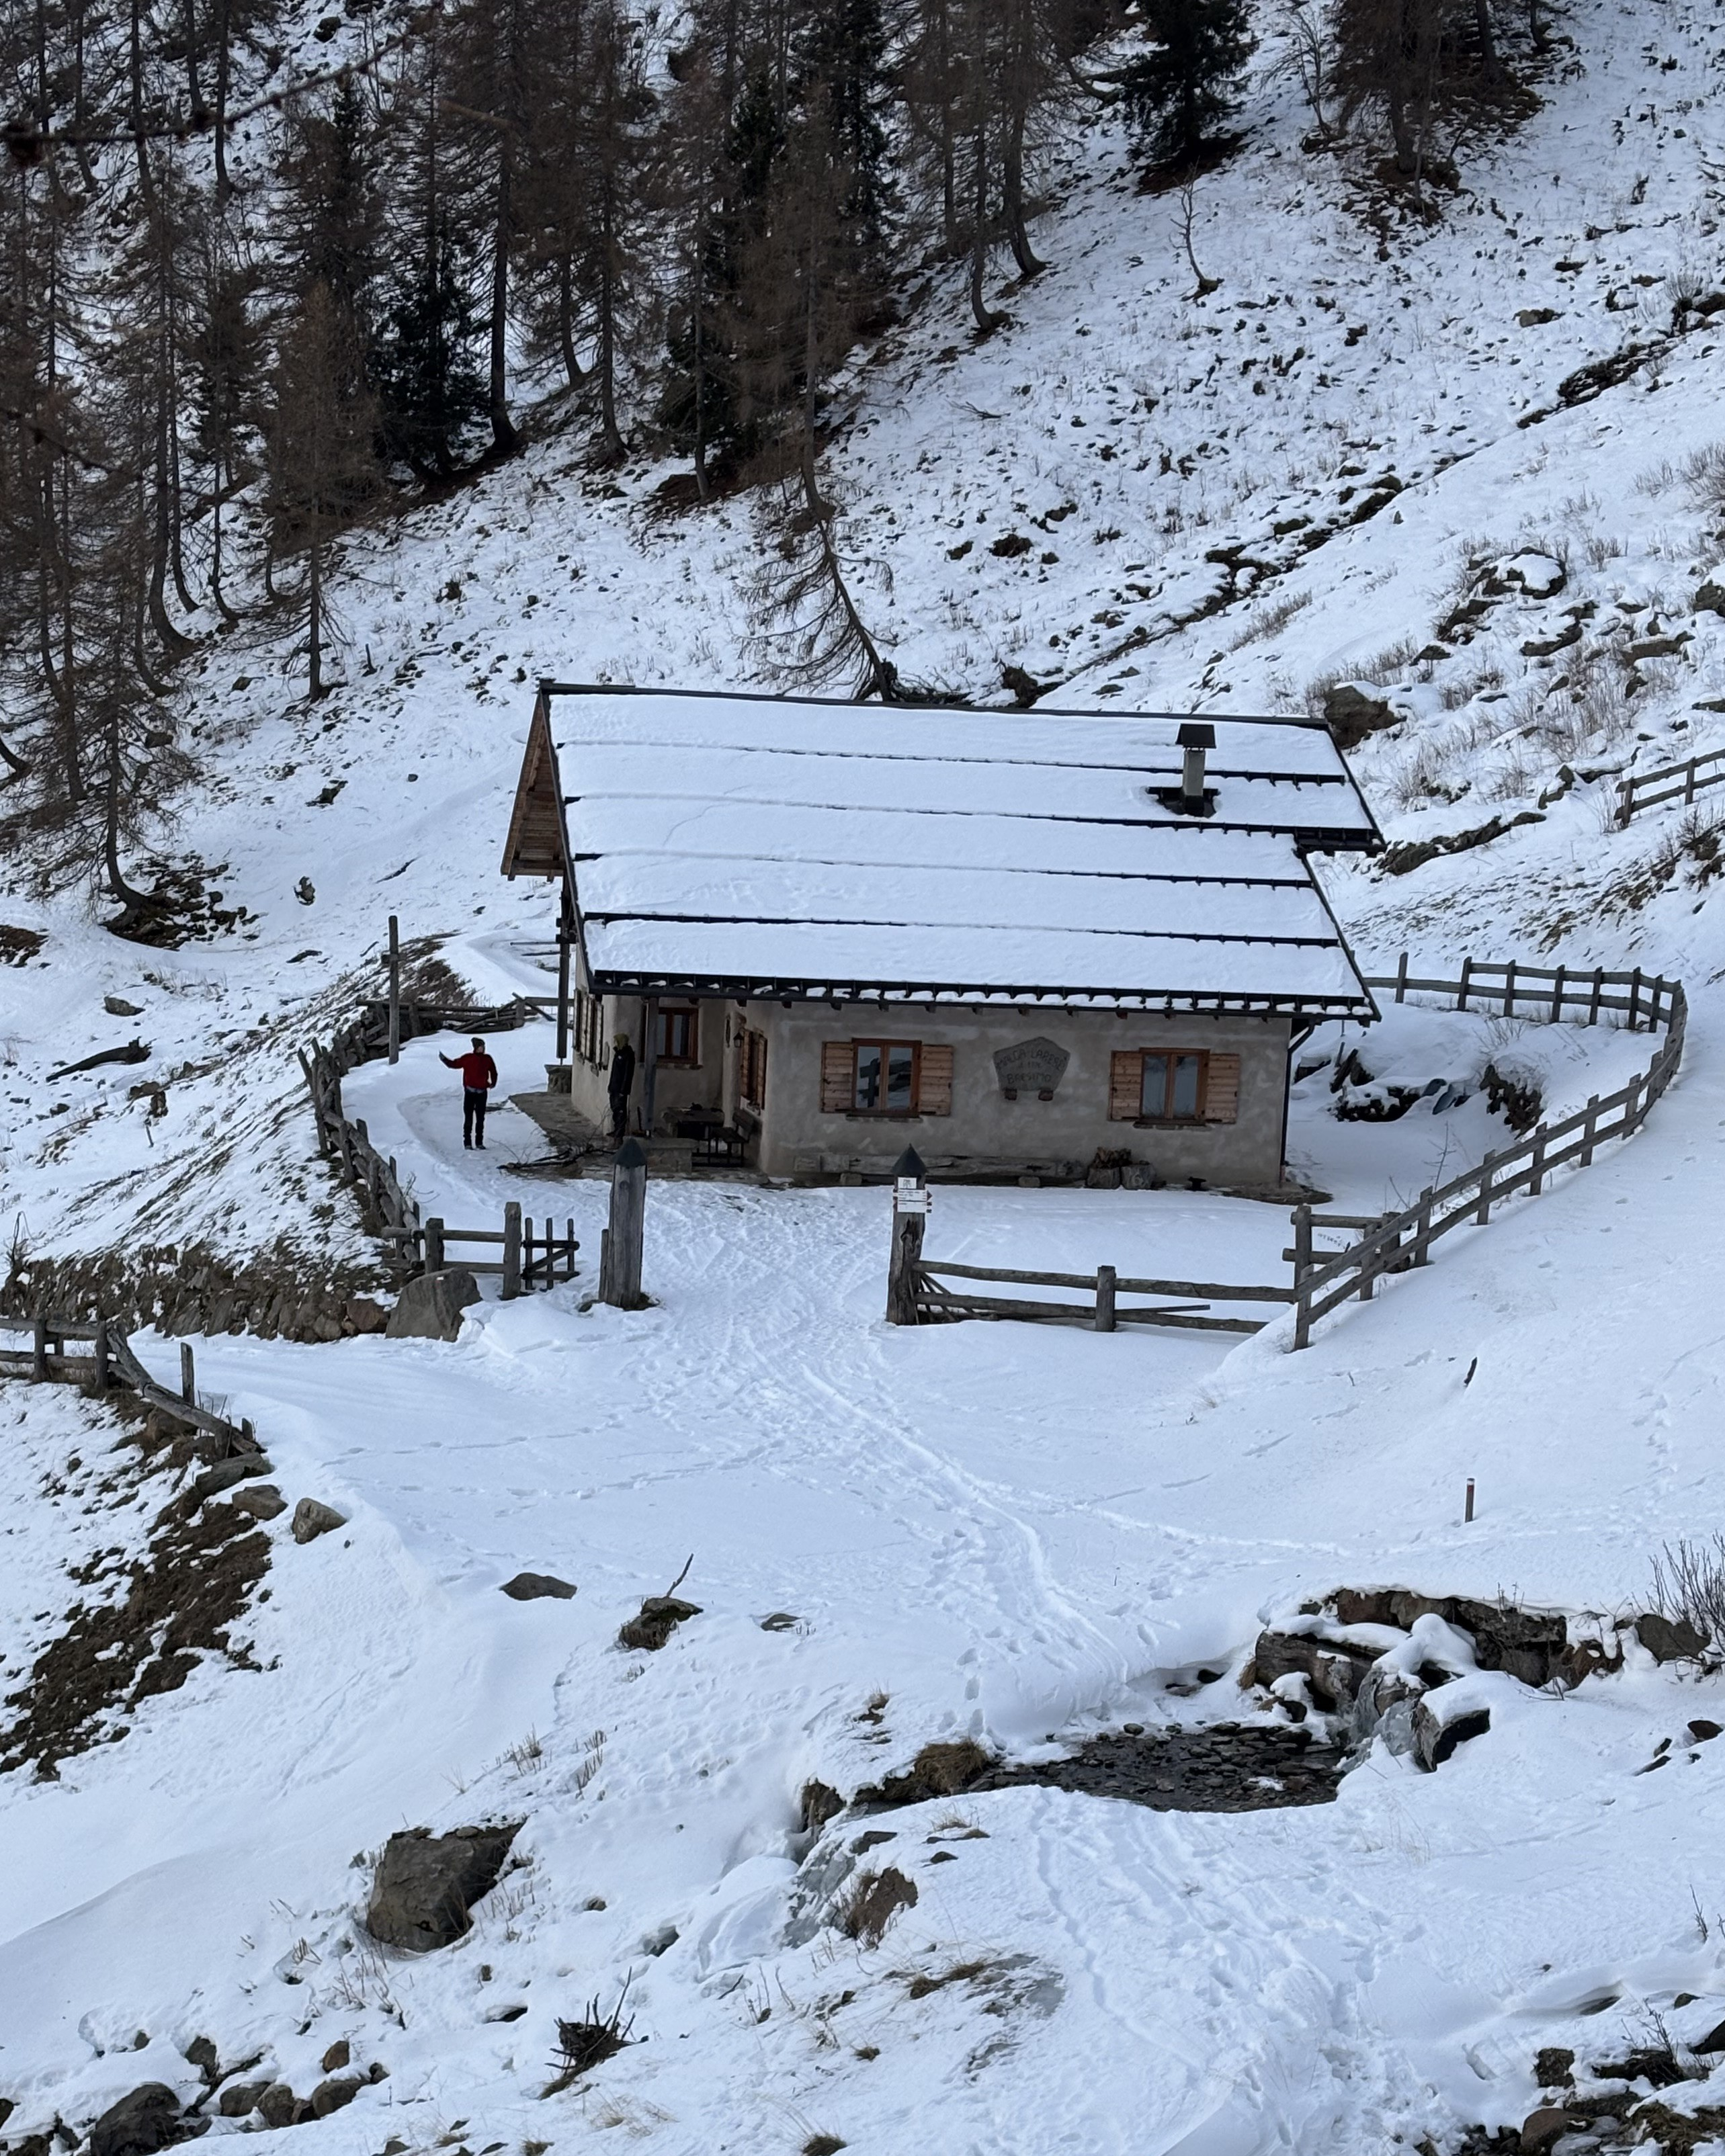
\includegraphics[width=\linewidth, frame]{images/bivacco.jpeg}
\end{minipage}%
\hfill
\begin{minipage}[t]{0.5\textwidth}
  \vspace{0pt} % forza l'allineamento in alto

  Regione\\
  \textbf{\large Trentino-Alto Adige}
  \\[1em] % Aggiunge una riga vuota qui
  Provincia/Comune\\
  \textbf{\large Trento / Bresimo}
  \\[1em] % Aggiunge una riga vuota qui
  Gruppo montuoso\\
  \textbf{\large Catena delle Maddalene}
  \\[1em] % Aggiunge una riga vuota qui
  Quota\\  
  \textbf{\large 1774 m s.l.m.}
  \\[1em] % Aggiunge una riga vuota qui
  Coordinate\\
  \textbf{\large \href{https://maps.google.com/?q=46.40299,10.92609}{46.40299° N, 10.92609° E}}
  \\[1em] % Aggiunge una riga vuota qui
  Apertura\\  
  \textbf{\large Gestito da Azienda agricola Giancarlo Carbonari, sempre aperto}

\end{minipage}

\subsection{Caratteristiche}
Il Bivacco Malga Laresè di sotto (bassa) è una struttura unica composta da stalla, alloggio per il pastore (casara), e  bivacco. È fornito sia di energia elettrica che di acqua calda solo nel periodo di apertura.

Il bivacco si sviluppa su due piani:
\begin{itemize}
    \item \textbf{Piano terra}: spazio principale della malga, un'ampia stanza con tavolo, panche, stufa a legna, lavandino e dispensa con diverso materiale (bombole, candele, acqua, risotti, giochi da tavolo, ecc.).
    \item \textbf{Piano superiore}: diviso in diverse stanze, con un totale di circa 20 brande con materasso. È presente anche un bagno con lavandino e water (ne sconsiglio l'utilizzo per mancanza di acqua nel periodo di chiusura).
    \item \textbf{Spazio esterno}: si presenta una stalla molto ampia e dietro al bivacco si può trovare una legnaia al tempo ben fornita. Il bivacco è poi "circondato" dal passaggio di 2 corsi d'acqua non molto grandi.
\end{itemize}

Sebbene sia presente una legnaia è comunque semplice ricavare la legna grazie al bosco che circonda il bivacco.

La vista dalla malga è spettacolare, si riesce a osservare tutta la vallata... E di notte quando il sole cala si crea uno spettacolo luminoso incredibile tra le vie della valle e il cielo stellato.

\section{Come ci siamo arrivati}
Abbiamo parcheggiato l'auto in uno \href{https://maps.google.com/?q=46.418194507125875,10.946478177557312}{spiazzo} lungo la strada e da li ci siamo incamminati. La salita è stata molto dura verso la fine, quando la neve era ormai molta anche sul sentiero. In circa 3 ore siamo arrivati al bivacco e malgrado quella non fosse la nostra meta originale abbiamo deciso di fermarci li per la notte. Il giorno dopo siamo scesi seguendo lo stesso percorso.

Lascio comunque i dati del giro completo che avevamo intenzione di fare, anche se poi è andata diversamente.

\begin{figure}[htbp!]
    \centering
    % Colonna di sinistra, allineata in alto
    \begin{subfigure}[t]{0.45\textwidth}
        \centering
        \vspace{0pt} % Forziamo l'allineamento in alto
        
\includegraphics[width=\textwidth]{images/sentiero_mapsMe.jpg}
        \caption{Sentiero su Maps.Me.}
        \vspace{2em}
        \textbf{Percorso fatto:}\\
        Giorno 1: 3.80 km $\leftrightarrow$, 590 m $\uparrow$, 10 m $\downarrow$
        Giorno 2: 3.80 km $\leftrightarrow$, 10 m $\uparrow$, 590 m $\downarrow$
    \end{subfigure}
    \hfill
    % Colonna di destra, allineata in alto
    \begin{subfigure}[t]{0.45\textwidth}
        \centering
        \vspace{0pt} % Forziamo l'allineamento in alto anche qui
        
\includegraphics[width=\textwidth]{images/sentiero_komoot.png}
        \caption{Sentiero su Komoot.}
        \vspace{3em} % Aggiunge un po' di spazio tra le due foto
        
\includegraphics[width=\textwidth]{images/profilo_altimetrico.jpg}
        \caption{Profilo altimetrico del percorso.}
    \end{subfigure}
    % Didascalia generale per l'intera figura
    \caption{Il sentiero e i dettagli del percorso.}
\end{figure}

% ==========================================================
%  Non ti scordar di me
% ==========================================================
\section{Non ti scordar di me}
\begin{tcolorbox}[colback=yellow!15!white, colframe=yellow!80!black]
\textbf{\textcolor{BurntOrange}{Ricorda: il bivacco è un bene comune. Il suo futuro dipende dal rispetto e dal senso civico dei visitatori. Usalo con cura e lascialo più pulito di come l'hai trovato.}}    
\end{tcolorbox}


\section{Esperienza personale}
Mi piacerebbe dire che questa era la meta che ci eravamo preposti ma così non è. Il nostro obiettivo era raggiungere il bivacco Pozze, poco più in su. Tuttavia, per colpa dell'ora tarda e della stanchezza generale, ci siamo dovuti fermare a questo bivacco.
Siamo arrivati al punto di partenza verso le 13.00 e la salita al bivacco è stata complessa. Il periodo invernale (siamo saliti il 31 dicembre per festeggiare capodanno insieme) non ha aiutato, era presente molta neve sul percorso al punto che senza ciaspole si sprofondava fino al ginocchio. La stufa presente nel bivacco riscalda molto bene l'ambiente, malgrado questo abbia comunque una dimensione notevole (non so dire le camere, noi abbiamo dormito tutto nel salone principale). Il giorno successivo abbiamo poi deciso di fare la stessa strada per tornare indietro.


\section{Alcune foto}

\begin{figure}[htbp!]
    \centering
    % Prima riga: Due foto (QUESTA È LA PRIMA FIGURA)
    \begin{subfigure}[b]{0.45\textwidth}
        
\includegraphics[width=\textwidth]{images/foto_sentiero.jpg}
        \caption{Sentiero.}
    \end{subfigure}
    \hfill
    \begin{subfigure}[b]{0.45\textwidth}
        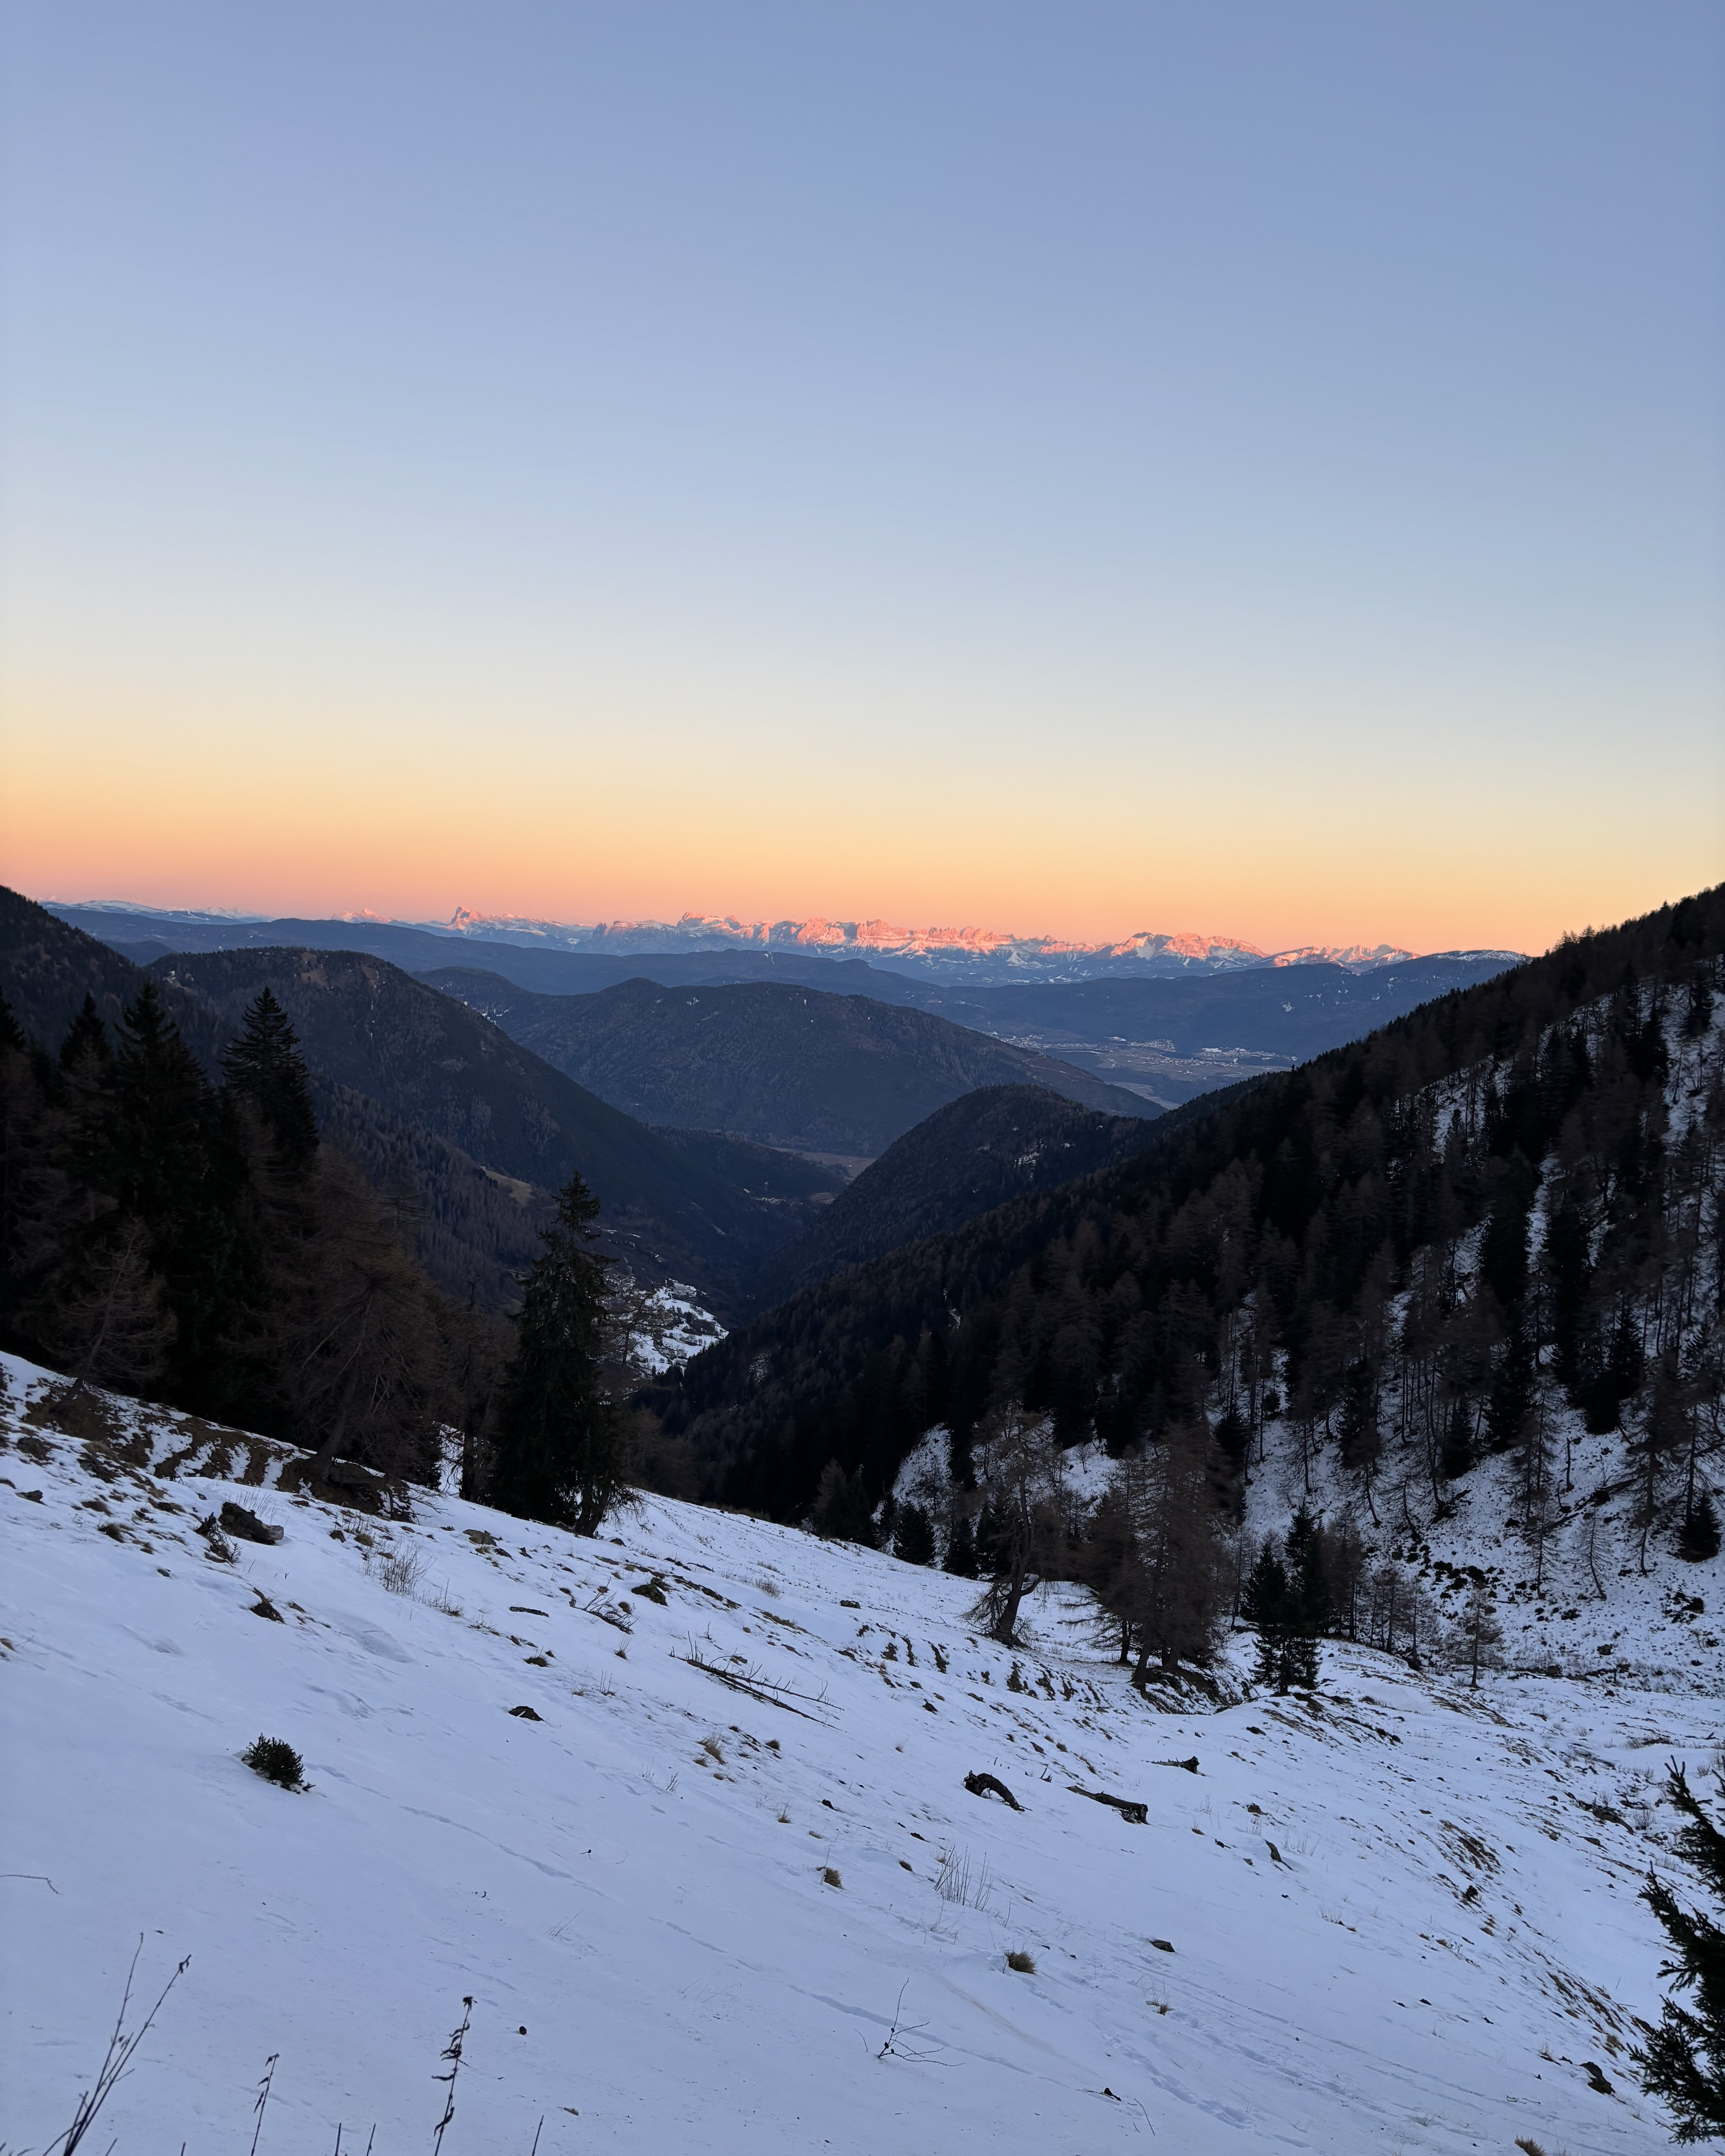
\includegraphics[width=\textwidth]{images/foto_paesaggio.jpeg}
        \caption{Paesaggio.}
    \end{subfigure}

\end{figure}

\begin{figure}[htbp!]
    \centering
    % Prima riga: Due foto (QUESTA È LA SECONDA FIGURA)
    \begin{subfigure}[b]{\textwidth}
        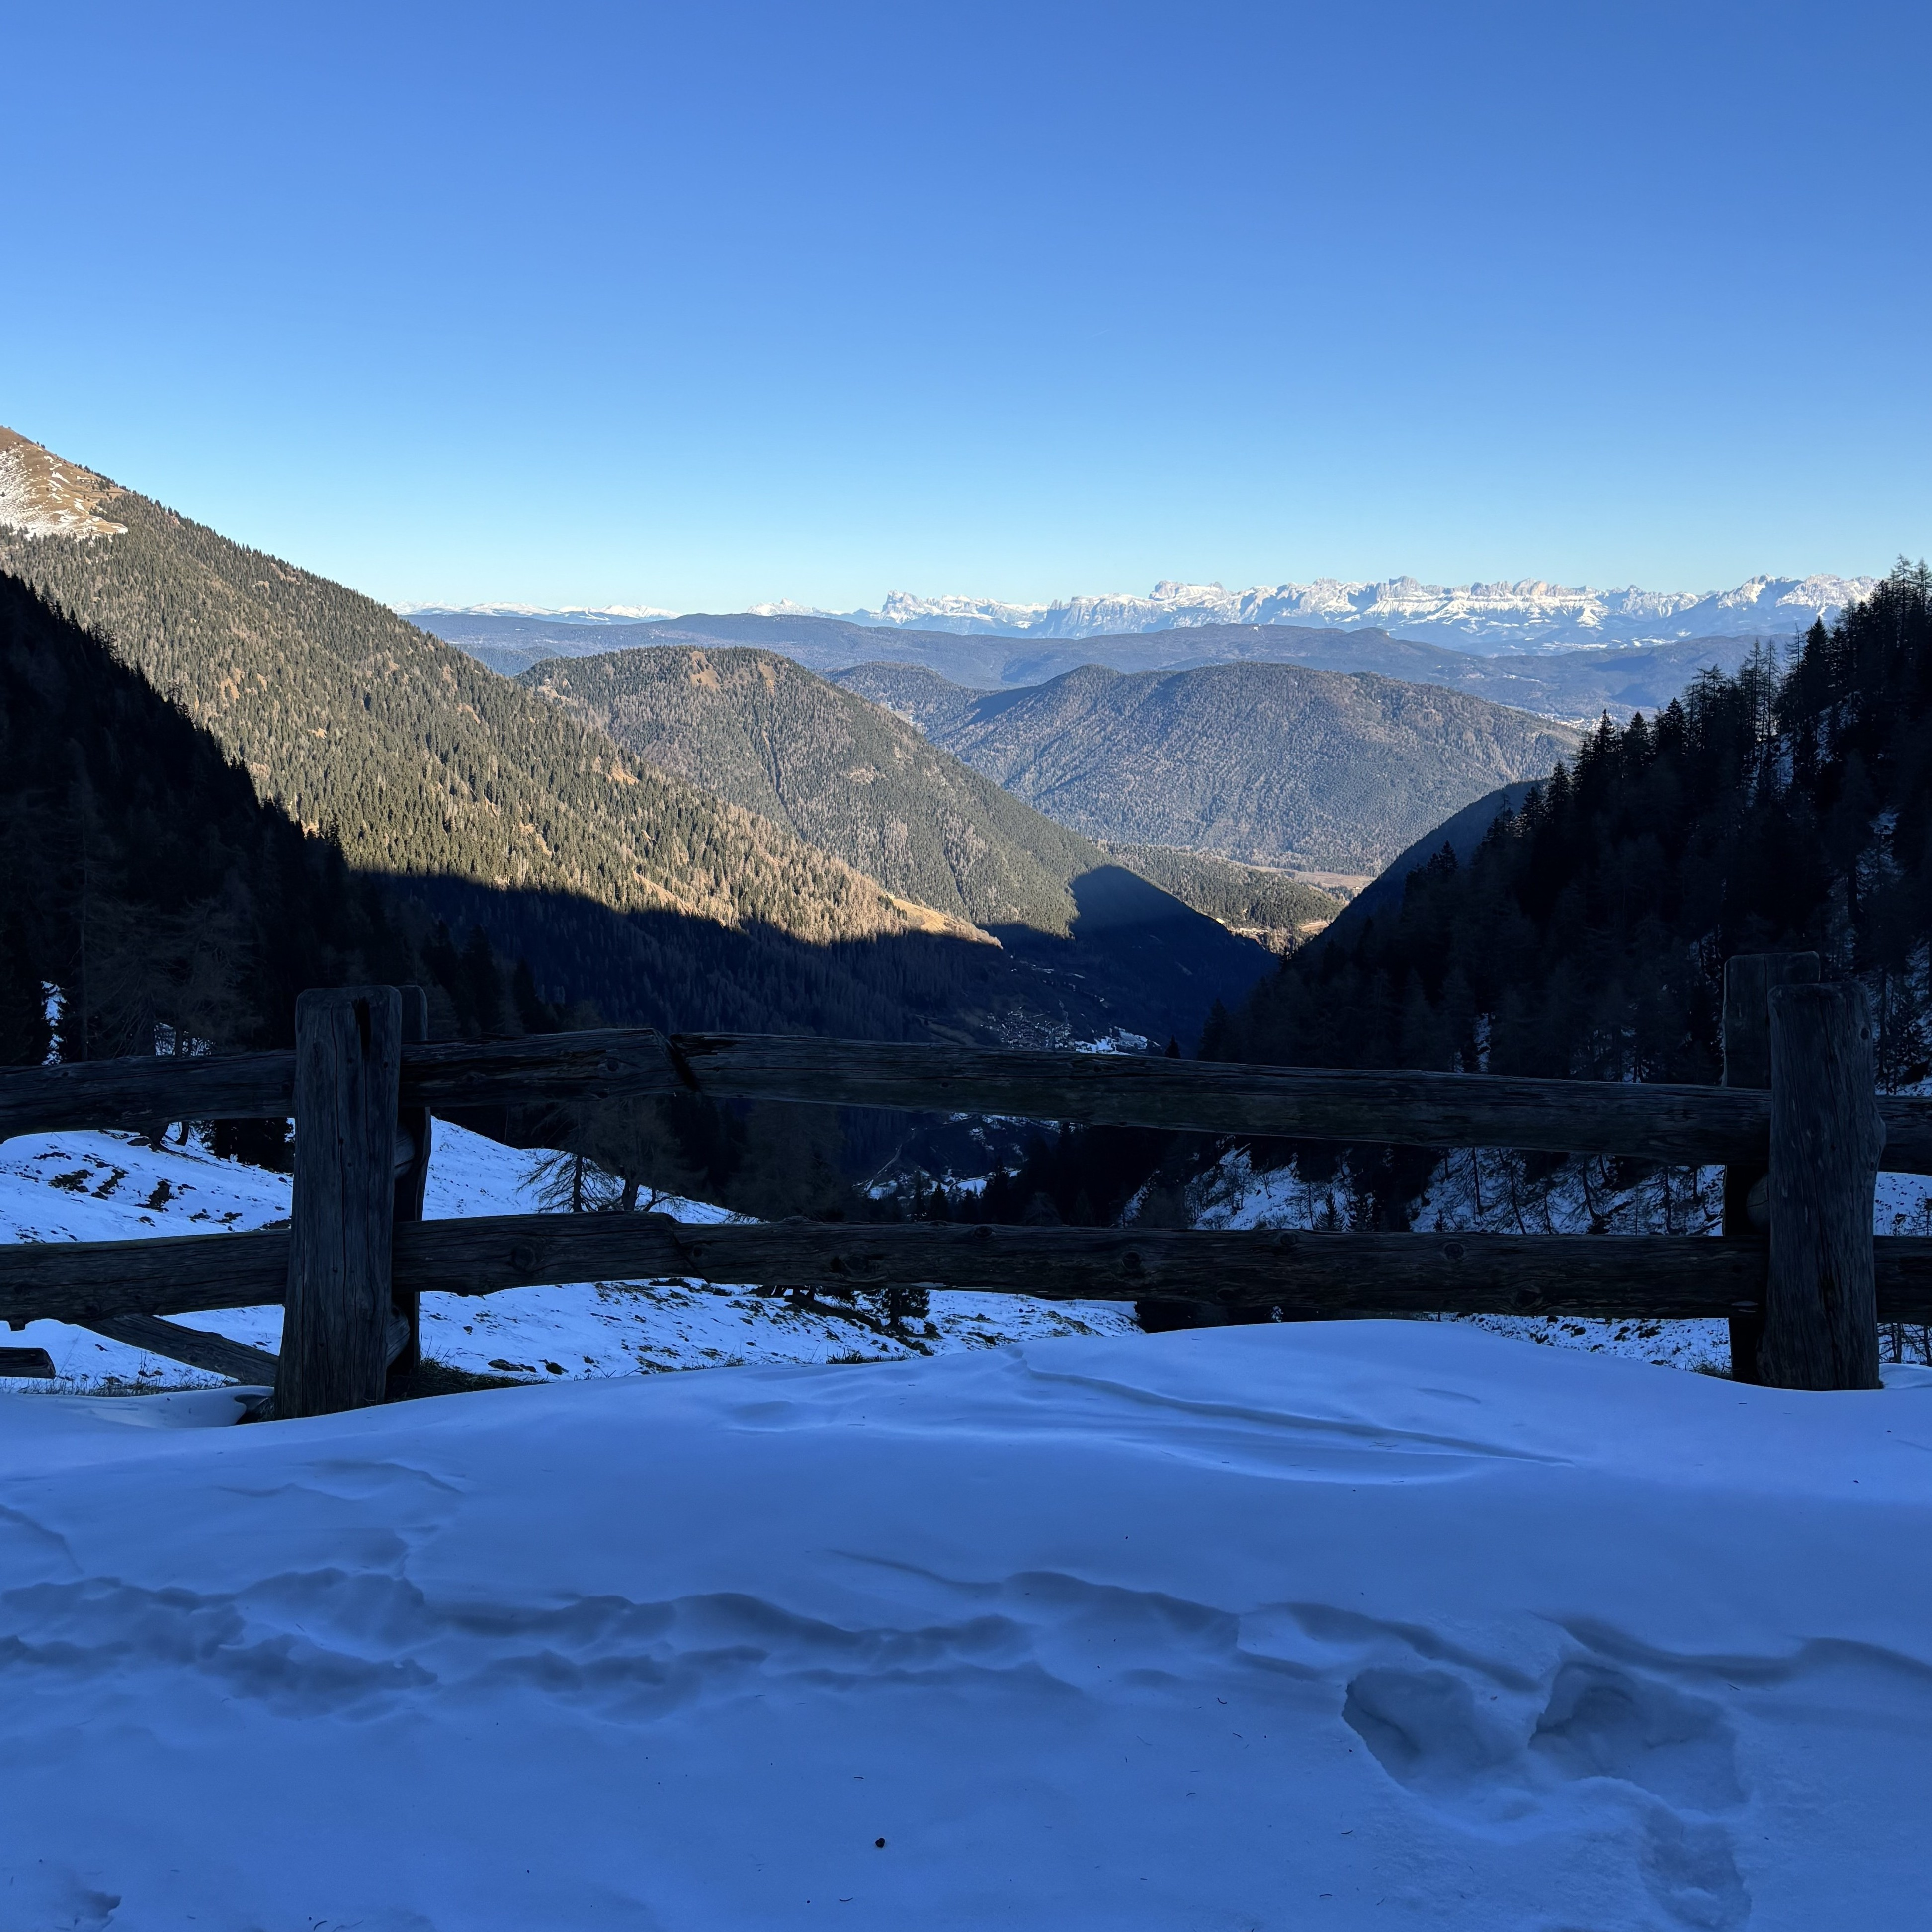
\includegraphics[width=\textwidth]{images/foto_vista.jpeg}
        \caption{Vista dal bivacco.}
    \end{subfigure}
   \hfill

    % setto il counter delle figure
    \setcounter{figure}{2}
    \caption{Selezione di fotografie del percorso e della vista dal bivacco.}
\end{figure}

\clearpage

\section*{Tabella riepilogativa delle caratteristiche}

\begin{tabularx}{\textwidth}{|l|X|}
\hline
\rowcolor{gray!15} \textbf{Caratteristica} & \textbf{Dettaglio} \\
\hline
Regione & Trentino-Alto Adige\\
Comune / Provincia & Trento / Bresimo \\
Gruppo montuoso & Catena delle Maddalene \\
Quota & 1774 m s.l.m. \\
Apertura & Gestito da Azienda agricola Giancarlo Carbonari, sempre aperto \\
Posti letto effettivi & 20 brande \\
Presenze in visita & 6 persone \\
Arredi & Tavolo, panche, stufa, cucina a gas \\
Acqua & \ding{51} - Lavandino interno con acqua (funzionante solo nel periodo di apertura) - corsi d'acqua \\
Servizi igienici & \ding{51} - Bagno (funzionante solo nel periodo di apertura)\\
Copertura telefonica & \ding{51} \\
Manutenzione / proprietà & Pubblico / Azienda agricola Giancarlo Carbonari / Comune \\
Visitato il & 31 dicembre 2024 - 1 gennaio 2025\\
\hline
\end{tabularx}


\end{document}
